\section* {1.1  LU -  разложение матриц}

\subsection{Постановка задачи}
Реализовать алгоритм LU -  разложения матриц (с выбором главного элемента) в виде программы. Используя разработанное программное обеспечение, решить систему линейных алгебраических уравнений (СЛАУ). Для матрицы СЛАУ вычислить определитель и обратную матрицу. 

{\bfseries Вариант:} 22

\begin{cases}
& 7x_1-5x_2+6x_3+7x_4 = 120 \\
& 8x_1-1x_2-9x_3+1x_4 = 31 \\
& -3x_1+8x_2+8x_3+8x_4 = 6 \\
& 2x_1-3x_2+6x_3-4x_4 = 25 \\
\end{cases}
% \pagebreak

\subsection{Результаты работы}
\begin{figure}[h!]
\centering
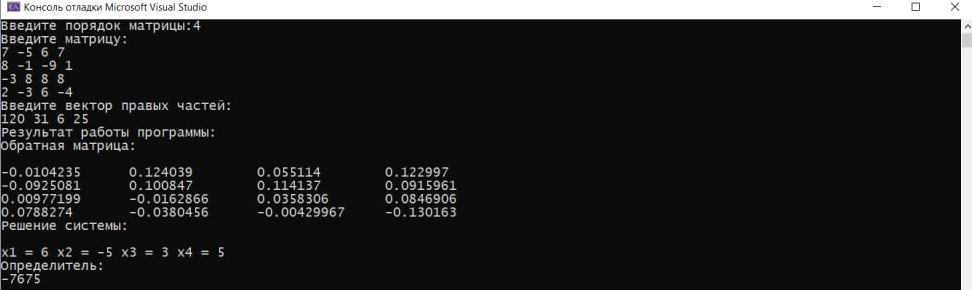
\includegraphics[width=.9\textwidth]{lab1.1}
\caption{Вывод программы в консоли}
\end{figure}

% \vfill

% \begin{figure}[h!]
% \centering
% 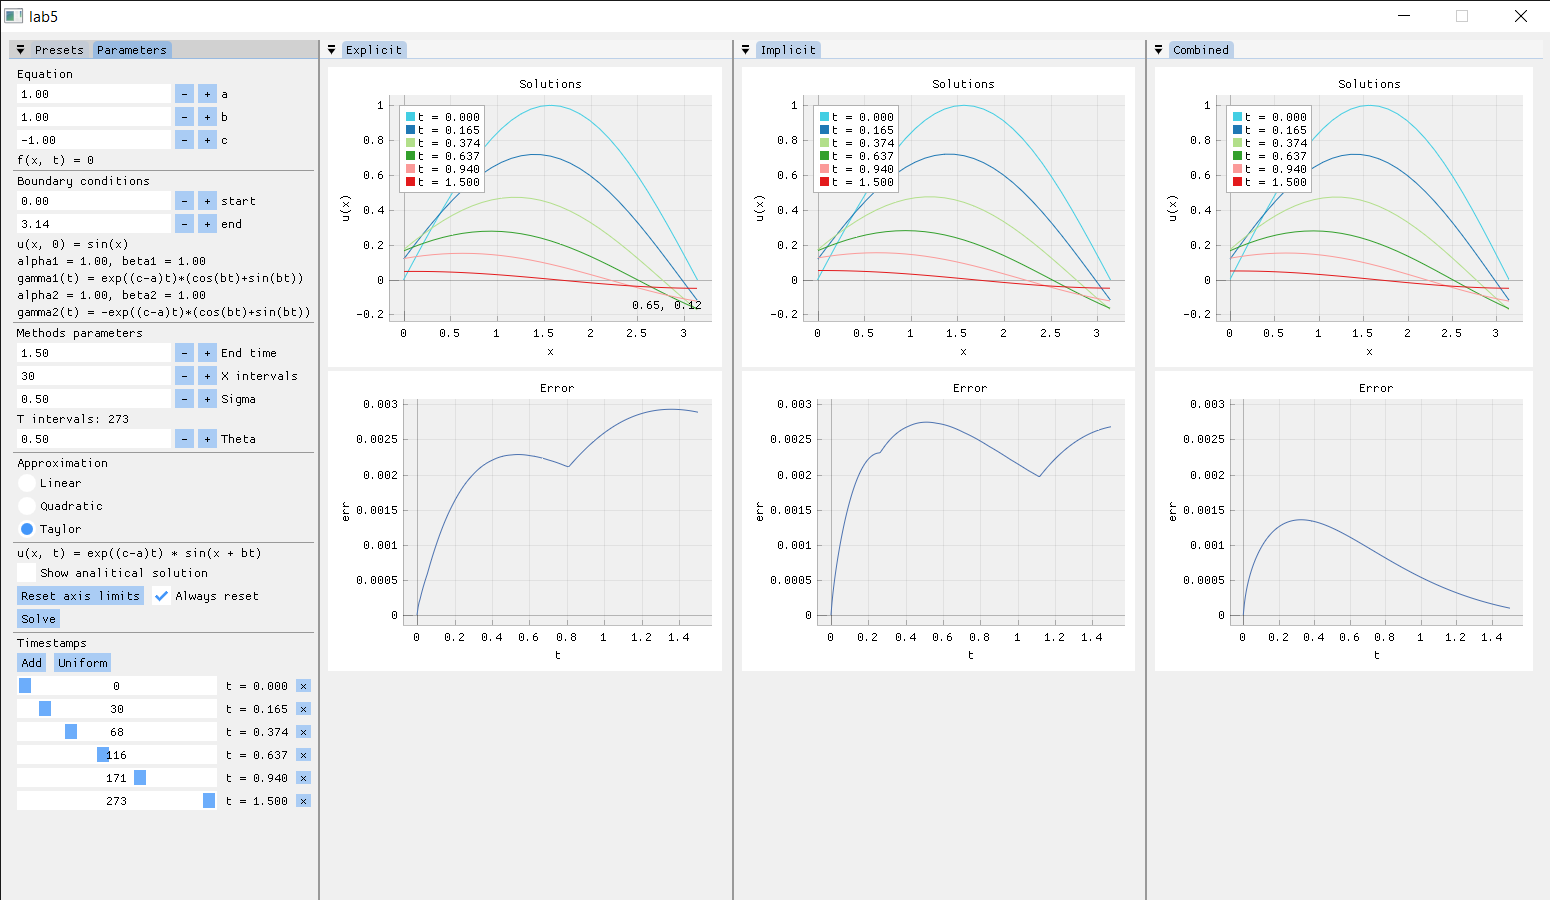
\includegraphics[width=.9\textwidth]{lab5_taylor}
% \caption{Решение с аппроксимацией граничных условий со вторым порядком}
% \end{figure}
\pagebreak

\subsection{Исходный код}
% \lstinputlisting[language=C++]{matrix.cpp}
% \begin{lstlisting}
\lstinputlisting{include/lab1_1.cpp}
\lstinputlisting{include/matrix.cpp}
\lstinputlisting{include/matrix.h}
% \end{lstlisting}
% \lstinputlisting{matrix.cpp}
% {../../include/matrix.cpp}
% \pagebreak
% \lstinputlisting[title=\texttt{parabolic\_pde.hpp}]{../../include/partial_differential/parabolic_pde.hpp}
% \pagebreak
% 